\begin{figure}[ht]
  \centering
  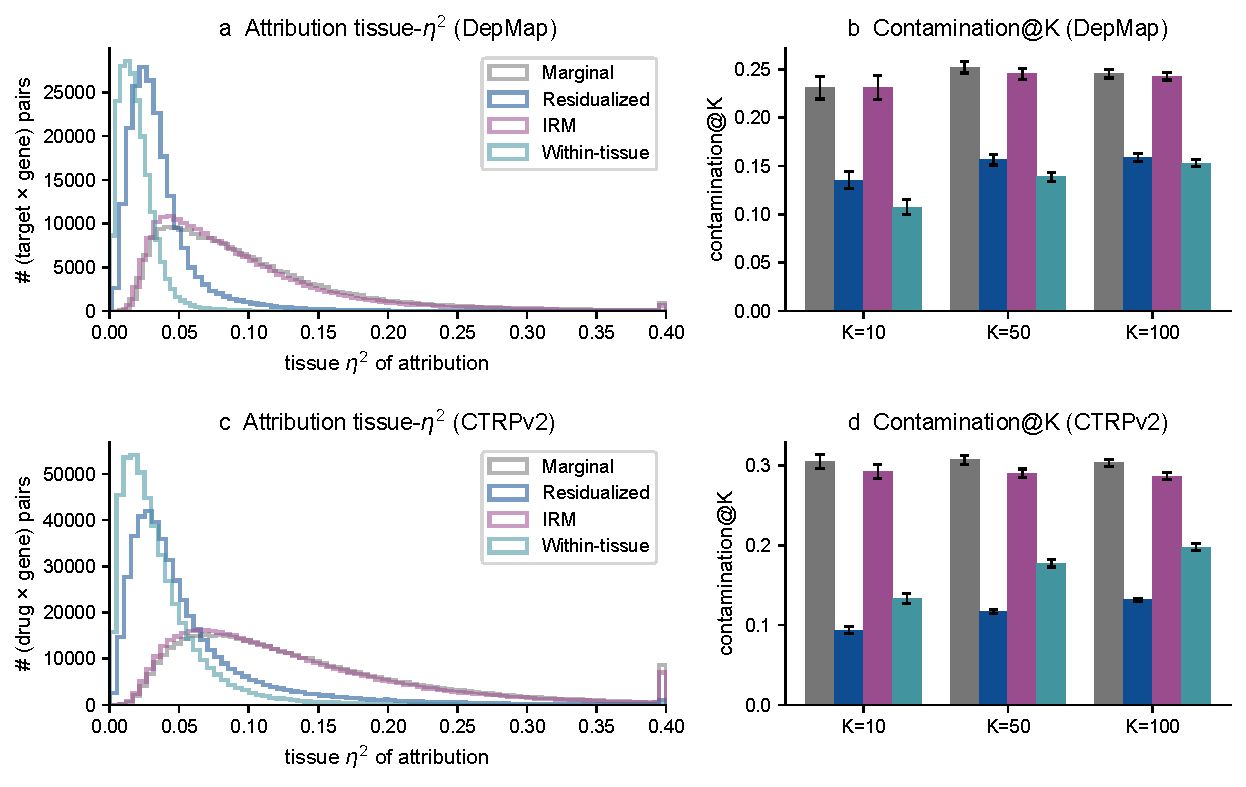
\includegraphics[width=\textwidth]{figures/fig06_ci_distribution.pdf}
  \caption{Deconfounding removes tissue signal from the attributions.
  (\textbf{a}, DepMap essentiality; \textbf{c}, CTRPv2 drug response) For every
  target/drug and gene,  we measure the tissue $\eta^2$ of the per-cell SHAP
  attribution (of a one-way ANOVA of $\phi$ against tissue); lower means
  less tissue signal in the attribution. Histograms show the per-(target/drug
  $\times$ gene) $\eta^2$ distribution for the four methods. Within-tissue SHAP
  and Residualized concentrate near zero, whereas Marginal and IRM exhibit more tissue-driven attributions.
  %
  (\textbf{b}, DepMap; \textbf{d}, CTRPv2) Top-$K$ tissue-marker enrichment.
  Contamination@$K$ is the fraction of a method's $K$ most-attributed genes that
  are tissue markers, i.e.,genes whose
  expression itself is strongly tissue-associated ($\eta^2_{\mathrm{expr}} >
  0.30$; $214$ of $1071$ genes for DepMap, $256$ of $1109$ for CTRPv2). Within-tissue
  and Residualized sit below chance at every $K$, so their top genes are depleted
  of tissue markers. Bars are mean $\pm$ standard error across targets/drugs.%
}
\end{figure}
